\documentclass{amsart}
\usepackage{amsaddr}
\usepackage{amssymb}
\usepackage[latin1]{inputenc}
\usepackage[swedish,english]{babel}
\usepackage{ifpdf}
\ifpdf
\usepackage[pdftex]{graphicx}
\usepackage{epstopdf}
\else
\usepackage[dvips]{graphicx}
\fi

\usepackage{caption}
\usepackage{subcaption}


% \usepackage{subfigure}
% \usepackage{sidecap}
\usepackage[pdftitle={Robin Eriksson - H3},
pdfauthor={Robin Eriksson},
pdffitwindow=true,
breaklinks=true,
colorlinks=true,
urlcolor=blue,
linkcolor=red,
citecolor=red,
anchorcolor=red]{hyperref}
% \usepackage{pdfpages}
\usepackage{algorithm}
% \usepackage{algorithmic}
\usepackage[noend]{algpseudocode}
\usepackage{dsfont}
\usepackage[numbers,sort&compress]{natbib}
\usepackage{appendix}
\usepackage[section]{placeins}
% **************************************************************************
\usepackage[margin=1.25in]{geometry}
\usepackage{subcaption}
% ***************************************************************************
\usepackage{microtype}
\usepackage{parskip}

\usepackage{listings}
\usepackage{color} %red, green, blue, yellow, cyan, magenta, black, white
\definecolor{mygreen}{RGB}{28,172,0} % color values Red, Green, Blue
\definecolor{mylilas}{RGB}{170,55,241}
% ***************************************************************************
\numberwithin{equation}{section}
\numberwithin{table}{section}
\numberwithin{figure}{section}

\theoremstyle{plain}
\newtheorem{theorem}{Theorem}[section]
\newtheorem{lemma}[theorem]{Lemma}
\newtheorem{proposition}[theorem]{Proposition}
\newtheorem{corollary}[theorem]{Corollary}
\newtheorem{conjecture}[theorem]{Conjecture}
% \newtheorem{algorithm}[theorem]{Algorithm}
% \newtheorem{criterion}[theorem]{Criterion}

\theoremstyle{definition}
\newtheorem{definition}{Definition}[section]
\newtheorem{assumption}[definition]{Assumption}
\newtheorem{convention}[definition]{Convention}
\newtheorem{example}[definition]{Example}
% \newtheorem{problem}[definition]{Problem}

\theoremstyle{remark}
\newtheorem*{remark}{Remark}
% \newtheorem*{note}{Note}
% \newtheorem*{notation}{Notation}
% \newtheorem*{summary}{Summary}
% \newtheorem{theorem}{Theorem}[section]
% \newtheorem{lemma}[theorem]{Lemma}

\renewcommand{\Pr}{\mathbf{P}}
\renewcommand{\P}{P}
\newcommand{\E}{\mathbf{E}}
\newcommand{\V}{\mathbf{V}}
\newcommand{\R}{\mathbb{R}}
\newcommand{\F}{\mathcal{F}}

% *** use these commands to write comments; they are easy to spot in the text!
\newcommand{\comment}[1]{\textcolor{blue}{\{#1\}}}
\newcommand{\margincomment}[1]{* \marginpar{\textcolor{blue}{*\{#1\}}}}


% *** todo list! ***
\usepackage{enumitem,amssymb}
\newlist{todolist}{itemize}{2}
\setlist[todolist]{label=$\square$}
\usepackage{pifont}
\newcommand{\cmark}{\ding{51}}%
\newcommand{\xmark}{\ding{55}}%
\newcommand{\done}{\rlap{$\square$}{\raisebox{2pt}{\large\hspace{1pt}\cmark}}%
  \hspace{-2.5pt}}
\newcommand{\wontfix}{\rlap{$\square$}{\large\hspace{1pt}\xmark}}



% **************************************************************************

\begin{document}

\title[]{Homework 3}

\author[R. Eriksson]{Robin Eriksson}
\email{\href{mailto:robin.eriksson@it.uu.se}{robin.eriksson@it.uu.se}}
% \address{Division of Scientific Computing \\
% Department of Information Technology \\
% Uppsala University \\
% SE-751 05 Uppsala, Sweden.}

% \subjclass[2010]{Primary: NNXMM; Secondary: NNXMM}

% \keywords{}

\date{\today}


\selectlanguage{english}
% \maketitle
Robin Eriksson; \href{mailto:robin.eriksson@it.uu.se}{robin.eriksson@it.uu.se}
\section{Neural Network as a Gaussian Process}\label{sec:gp}
We aim to numerically verify that Neural networks at the
initialization tend to Gaussian Processes (GP) in the infinite width
limit, as stated in~\cite{NEURIPS2018_5a4be1fa}.

We construct a neural network with 4 hidden layers and a width of
1000.  (additional parameter: $\beta = 0.1$, samples for kernel
estimation $= 1000$). For that network we do two things, first we only
train the final layer (red lines) and then we estimate the GP using
the untrained hidden layers (grey lines) to approximate a kernel. The two steps are
independent. The result is seen in \ref{fig:NNasGP}. Red and grey are
similar in shape and the tigtest credible intervals cover the reds.


\section{Neural tangent kernel}\label{sec:ntk}
Next, \cite{NEURIPS2018_5a4be1fa} also showed that the wide nets (tend
to infinity), gradient descent can be done by using a ``Neural Tangent
Kernel'' (NTK) which can make the training deterministic. We continue as
before and confirm this result numerically.

We use the same network set-up, but now also define the learning rate
$= 1$ and epochs $= 1000$. First we train the network by classical
gradient descent for multiple seed (red lines), then for comparison we
approximate the NTK trained network (grey lines). The result is seen
in \ref{fig:NTK}. The grey and red lines are close to each other again
telling us that the statement seems to be true.

Comparing \ref{fig:NNasGP} and \ref{fig:NTK} we can note that the
trained networks interestingly find shortcuts between the observations
whilst the untrained seems to be more smooth --- which makes sense.

\begin{figure}[h]
  \centering
  \begin{subfigure}[b]{0.45\textwidth}
    \centering
    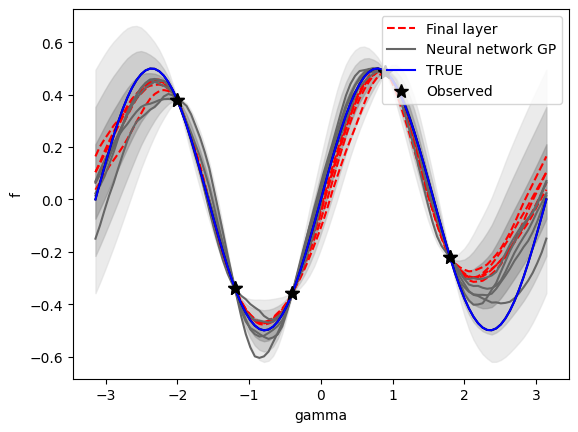
\includegraphics[width=1.2\textwidth]{part1}
    \caption{Part 1}
    \label{fig:NNasGP}
  \end{subfigure}
  \hfill
  \begin{subfigure}[b]{0.45\textwidth}
    \centering
    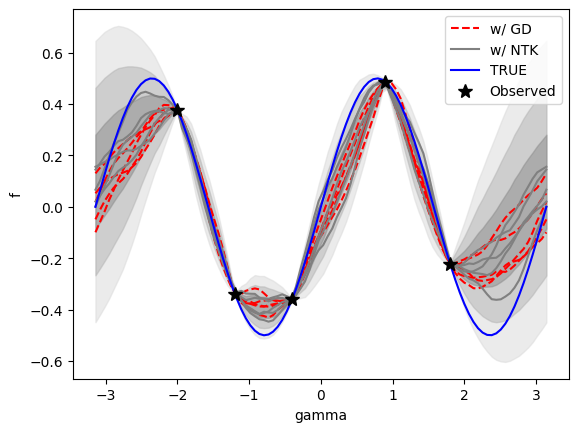
\includegraphics[width=1.2\textwidth]{part2}
    \caption{Part 2}
    \label{fig:NTK}
  \end{subfigure}
  \caption{Output figures from part 1 and 2. Both include shaded
    regions, these correspond to the credible intervals of the
    Gaussian process (part 1) and NTK Gaussian distribution (part
    2). Both of them are related to the grey solid lines which are
    samples from said distribution. Additionally, both figures include
    the true function (blue line) and the five observations (black
    stars). }
  \label{fig:results}
\end{figure}


\bibliographystyle{plain}
\bibliography{report3}

\end{document}
